%!TEX root = ../pres.tex


\begin{frame}
	\frametitle{Policy Iteration}
	
	\onslide<1->{\textbf{Policy Iteration:} Given access to the MDP, use policy evaluation to iteratively serach for better policies!}
	\begin{itemize}
		\item<1-> Choose a policy at random, $\pi
		$.
		\item<2-> Alternate between
		\begin{itemize}
			\item<2-> Evaluate policy $\pi \to V^\pi$.
			\item<3-> Set new policy to be greedy policy for $V^\pi$
			\begin{equation*}
			\begin{aligned}
				\pi(s) & := \argmax_a \mathbb{E}\left[R(s,a) + \gamma V^{\pi}(s')\right] \\
						& := \argmax_a Q^{\pi}(s, a)
			\end{aligned}
			\end{equation*}
		\end{itemize}
	\end{itemize}
	\onslide<4->{ \emph{Note: Learn $Q^{\pi}$ using Q-learning without $\argmax.$} 
				\begin{equation*}
					Q^{\pi}(s_t,a_t) = r(s_t, a_t) + \gamma Q^{\pi}(s_{t+1}, \pi(s_{t+1})
				\end{equation*}}

\end{frame}


\begin{frame}
  \frametitle{Policy Iteration}
  \textbf{Example: Deep Determisitic Policy Gradient}
  \begin{enumerate}
    \item Actor neural network $\pi_\theta: \scripts \to \scripta$
    \item Critic network $Q^\pi: \scripts \times \scripta \to \mathbb{R}$
    \item Performance of $\pi$ is $Q^\pi(s_t, \pi(s_t))$. \textbf{Maximize performance!} $\nabla_\theta Q^{\pi}(s_t, a_t) = \nabla_a Q^\pi(s_t,a) \cdot \nabla_\theta \pi_\theta(s_t)$
  \end{enumerate}
	\begin{center}
	  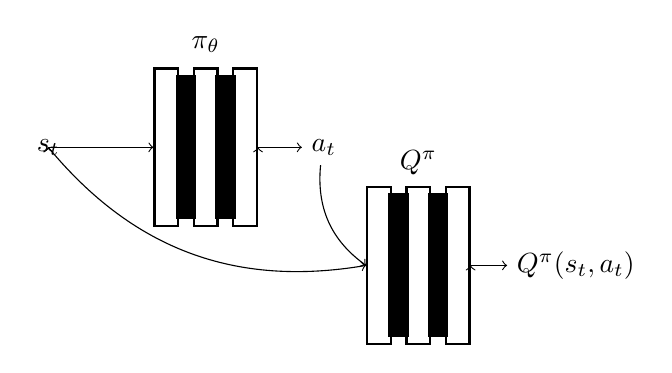
\begin{tikzpicture}
	\node[rectangle] at (0,0)  {$s_t$};
	\node[rectangle] at (1.75,0) [draw,thick,minimum width=0.2cm,minimum height=1.8cm, fill=black] (BC1) {};
	\node[rectangle] at (2.25,0) [draw,thick,minimum width=0.2cm,minimum height=1.8cm, fill=black] (BC2) {};
	\node[rectangle] at (1.5,0) [draw,thick,minimum width=0.3cm,minimum height=2cm] (B1) {};
	\node[rectangle] at (2,0) [draw,thick,minimum width=0.3cm,minimum height=2cm] (B2) {};
	\node[rectangle] at (2.5,0) [draw,thick,minimum width=0.3cm,minimum height=2cm] (B3) {};
	\node[rectangle] at (3.5,0) (action) {$a_t$};
	\draw[->] (B3.east) edge (action.west);
	\node[rectangle] at  (2,1.3) {$\pi_\theta$};
	\draw[->] (0,0) edge (B1);

	\node[rectangle] at (2.7+ 1.75,-1.5) [draw,thick,minimum width=0.2cm,minimum height=1.8cm, fill=black] (QC1) {};
	\node[rectangle] at (2.7+ 2.25,-1.5) [draw,thick,minimum width=0.2cm,minimum height=1.8cm, fill=black] (QC2) {};
	\node[rectangle] at (2.7+ 1.5,-1.5) [draw,thick,minimum width=0.3cm,minimum height=2cm] (Q1) {};
	\node[rectangle] at (2.7+ 2,-1.5) [draw,thick,minimum width=0.3cm,minimum height=2cm] (Q2) {};
	\node[rectangle] at (2.7+ 2.5,-1.5) [draw,thick,minimum width=0.3cm,minimum height=2cm] (Q3) {};
	\node[rectangle] at (2.7+ 2,-1.5 + 1.3) {$Q^\pi$};
	\draw[->, bend right] (0,0) edge (Q1.west);
	\draw[->, bend right] (action) edge (Q1.west);
	\node[rectangle] at (2.7+ 4,-1.5) (critic) {$Q^{\pi}(s_t, a_t)$};
	\draw[->] (Q3.east) edge (critic.west);
	\end{tikzpicture} 
	\end{center}
\end{frame}


\begin{frame}
	\frametitle{$\ $}
	\begin{center}
	\textbf{and many more...}\\
		Papers and links to descriptions of other algorithms will be posted on github.com/mlberkeley/bootcamp.
	\end{center}
\end{frame}